\section{Spatial Data Infrastructure}
% Introduce the topics at hand 

% This chapter offers a theoretical background on the ideas needed to assess the quality and openness of the SSDI. It starts out with a summary on the SDI in general and its three generations. Next, the Open SDI theory is covered, and the cross-European directives that gave birth to it, along with the role national mapping agencies play in an Open SDI. Finally, this knowledge is used in order to choose an assessment framework, to precisely measure in which ways the NSDI of Scotland is in accordance to this theory. 

\subsection{SDI Theory}

\subsubsection{The SDI} 

A Spatial data infrastructure (SDI) refers to a system of acquiring, sharing and using spatial data. It is a full framework of technologies, policies, and standards to continuously facilitate this \citep{status_national_open_SDI_2020}. 

\begin{figure}
    \centering
    \graphicspath{ {images/} }
    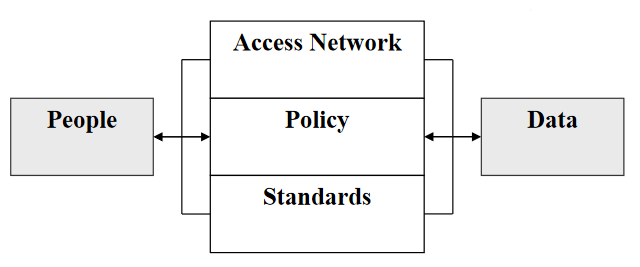
\includegraphics[width=12cm]{SDI_elements}
    \caption{The main elements of an SDI}
    \label{fig:SDI_elements}
\end{figure}

% COMMENT: CHANGE THIS TO 6 MAIN ELEMENTS, ADD GOVERNANCE 
An SDI covers 5 main elements (Figure \ref{fig:SDI_elements}): Stakeholders, Data, Policy, Standards, and an Access Network \citep{status_national_open_SDI_2020}. All of this is managed by a sixth element, called 'Governing'. The main purpose of an SDI is to connect the 'Stakeholders' and 'Data'. This connection is coordinated by means of technical solutions (Access Network), Legal solutions (Policy), and standardization.   

\subsubsection{SDI Evolution}

Three distinct generations of SDI can be distinguished, as stated by \citet{expanding_knowledge_base}. A First Generation SDI refers to an SDI which is data-driven. The SDI is in place mainly to facilitate efficiency among producers of geo-data. 

A second generation SDI improves upon this by focusing on process. It recognises that an SDI which is not being utilized by users is not an effective SDI, however efficient it may be for producers \citep{geo1009_course}. Meeting user needs becomes an objective, along with a broader societal perspective on the goal of 'value creation'. Finally, a second generation SDI recognises that spatial data contains a certain intrinsic value, as in it should be available to anyone \citep{geo1009_course}. This is why a second generation SDI aims for effective communication between the datasets \& non-experts users.

A Third generation SDI goes even further. Such an SDI revolves not only around process, but product as well. The goal of the SDI shifts to truly empowering the users, and to further remove the distinction between producer and user. These 'produsers' can in turn be used to crowd-source the acquisition of geo-information \citep{geo1009_course}. 

\subsection{Cross-European Directives}

On a European level, various efforts have been made to unify datasets across the borders of EU member-states. Two of the most recent developments have been the INSPIRE directive, aiming to improve the access and sharing of datasets which relate to environmental issues (either directly or indirectly) \citep{inspire_directive_2007}, and the more recent PSI Directive, which aims to facilitate the re-use of public sector information datasets across all the member-states by harmonizing conditions and removing the major barriers \citep{psi_directive_law_2011}. The latest development by the European Commission comes in the form of the Open Data Directive, which is built upon this PSI Directive \citep{open_data_directive_2019} and improves it by addressing the various barriers which exist towards creating a truly open (fourth generation) SDI \citep{eucommission_psiToOpen}.

It should be noted that Scotland has its own INSPIRE Directive regulations (as opposed to the rest of the UK - England, Wales and Northern Ireland), with its own amending legislation \citep{Inspire_amendment_debate_2019}. Thus, it has a somewhat independence when it comes to this. In 2019, the Scottish Ministers modified the the Scottish Statutory Instrument (which is a set of laws under the Scottish Government - \citep{guide_SSIs}) which prepared the country for Brexit by maintaining the alignment of the regulations of the Public Sector Information to those in the EU \citep{Inspire_amendment_law_2019}

\subsection{Open SDI} %Alex

% BASTIAAN: STRONGLY MENTION THE TWO COMPONENTS OF AN OPEN SDI : OPEN DATA & OPEN PARTICIPATION
% - Explain the role of open-data in OPEN SDI  
% - The concept of Open SDI - i.e. no limited to Open data only, but addressing the infrastructure components as well 

The emphasis by the EU on transparency, open data, High Value Datasets, and the re-use of public sector information necessitates that the NSDIs of member states evolve beyond the previously defined third generation SDI. This is where the theory of 'Open SDI' comes into play. The newly coined 'Open SDI' can be seen as a fourth generation SDI \citep{geo1009_course}. It requires two concepts to function properly: Open Data \& Open Participation. The idea behind the open SDI is that public administration agencies will make governmental data (which includes geo-data) available without constraints to the public (Open Data), and at the same time, grant the status of key-active stakeholders in the data infrastructure to various non-governmental users, such as average citizens, NGOs, universities, research institutions, and the private sector (Open Participation) \citep{emergance_open_data_2018}.

\subsubsection{Open Data} 

Open data is defined as "data that anyone can access, use and share" \citep{euro_data_portal_open_data}. Accessibility refers to whether or not the data is available to the public, perhaps on a online platform. Usage implies that the data in question is available in a common, understandable format. Sharing consists of licensing. Open data should legally offer the possibility to re-use and re-purpose the data, including for various commercial purposes. 

In essence, the lack of imposed restrictions is what makes data truly open. If, for example, there is a non-commercial license applied on the data, then it is considered as restricted, and thus no longer open.

\subsubsection{Open Participation}

% "the users are involved the most, but the least considered" (mcLaughlin and Nichols, 1994)

In first generation SDIs, the users are only passive recipients of geodata. Open Participation stands for the exact opposite. In an Open SDI, the role of the user must be active, so that the difference between user and producer begins to erode. This lead to the term "produser" \citep{status_national_open_SDI_2020}. Users who heavily invest in the SDI like this will in turn create data flow and activity in general. \citep{towards_user_oriented_open_data_strateg_2018}. There are different levels of involvement which an SDI can strife for, from non-participation to complete user control. At this level, the decision-making process is fully administered by the user, and are granted authority over decisions such as controlling the budget or determining the direction of the SDI \citep{towards_user_oriented_open_data_strateg_2018}. Of course, in-between these two extreme situations, there is a spectrum of possible roles which the users can take. 

\subsection{Open SDI: Role of NMA and Parcel Dataset}

Cadastral parcel datasets are considered high-value datasets (HVDs), due to the fact that they "provide a link between the land parcel, its ownership or other rights and potentially other information held in a national cadastral database (such as property value)." \citep{HVD_parcels_2020}. Due to this fact, the organizations which administer these land registries, such as a Cadaster agency or the National Mapping agency have a significant role in the development and operation of an SDI. 

In Scotland, the parcel datasets are administered by the Registers of Scotland, which is "the non-ministerial government department responsible for compiling and maintaining 20 public registers" \citep{scot_gov_ros_description}. Also according to the description provided by the Scottish government, these different registers relate to land, property, and other legal documents.

With the focus of an Open SDI in mind, European mapping agencies have been encouraged, through the Open Data PSI directive \citep{open_data_directive_2019}, to make certain HVDs from the public sector open. Thus, these agencies will be regarded as a main actor in this development. 

The importance of the RoS and its HVD potential must be reflected in our assessment on the openness of the SSDI. Thus, besides applying the assessment framework to the entire SSDI, we will also apply them specifically to the parcel dataset. 

\subsection{Assessment Framework}

To answer the research question, we will need to address how well Scotland's NSDI relates to this theory of open SDI. We require a concrete assessment criteria to judge if the NSDI can be regarded as an Open SDI, and if not, how far off it exactly is. This chapter states our assessment framework, and how we derived it. 

\subsubsection{Existing frameworks}

Multiple (Open) SDI assessment frameworks exist. We regarded the frameworks used by \citet{assessing_openness_SDI_2018}, \citet{mulder}, and \citet{olausson}. 
To judge the validity of the assessment criteria of these frameworks, \textit(assessment criteria of the assessment criteria) are needed. The SMART-paradigm \citep{smart_1981} was therefore used. The elements of SMART \textit{(Specific, Measurable, Assignable, Realistic and Timely)} state that criteria should be clearly measurable, relevant, and achievable. In addition, we also judged the existing frameworks based upon \textit{Completeness}, for the framework should cover both the Open data aspect, as well as the open participation aspect of an Open SDI. 

% FIGURE: VAN Vancauwenberghe CRITERIA
the 'new open SDI assessment framework', as presented in \citet{assessing_openness_SDI_2018}, is created to reflect recent open data developments. It correctly covers both the Open Data \& Open participation aspects of an Open SDI. But, according to our assessment, indicators like \textit{"Assessment of the easiness for which data could be found using a web search (score: low or high)"} or \textit{"Existence of clear vision and/or strategic document on open spatial data (score: low, medium or high")} fail to be properly measurable. A clear vision is important, but the clarity of a vision is a very difficult phenomenon to objectively measure, and too open to interpretation. The dimension of data, however, contains indicators which are more clearly stated, and binary in terms of scoring. 

% FIGURE: MULDER'S CRITERIA
The assessment framework stated in \citet{mulder}, is more straightforward in this regard. Most criteria state a certain phenomenon e.g., \textit{"The data can be downloaded without registration"}, which can have a clear \textit{"No / Yes"} score. However, this list of criteria  fail to access the user participation aspects upon which an open SDI relies. 

% FIGURE: OLAUSSONS'S LEVELS OF PARTICIPATION
Thirdly, we regarded the Levels of Participation, as stated in \citet{olausson}. What makes this 'tier-list' useful, is the fact that it clearly lists aspects which need to be present in every level of participation. This turns 'participation' into something discrete and measurable. But, for this tier list to be included into a general open SDI framework, different modes of participation (local level-, national level-, policy- or technical-) will have to be included.  

\subsubsection{Our Framework}

Because none of the existing frameworks covered the entire scope of an Open SDI, and because not all criteria were clearly measurable, it was necessary to create a new framework. This framework is based upon the best aspects of the the mentioned frameworks, and focuses on measurability \& completeness. 

% ------------------------------------------------------------

% FIGURE: OUR OPEN SDI ASSESSMENT FRAMEWORK 

% ---------------------------------------------------------------

The Open Data criteria are directly taken from Mulders, with some minor changes to improve the measurability, and to make the scoring system more uniform. Specific criteria judging the completeness of specifically the parcel dataset, are added from Vancauwenberghe. Concerning the open participation criteria, we took liberties to create new assessment elements, based upon the 6 SDI components stated in \citet{towards_user_oriented_open_data_strateg_2018}. These express the different modes of open participation. An SDI can have high levels of user participation regarding the creation of datasets, but almost no participation regarding policy-making. To properly score \& measure these criteria, we use Olausson's levels of participation. 

\begin{figure}
    \hspace*{-3cm}
    \graphicspath{ {images/} }
    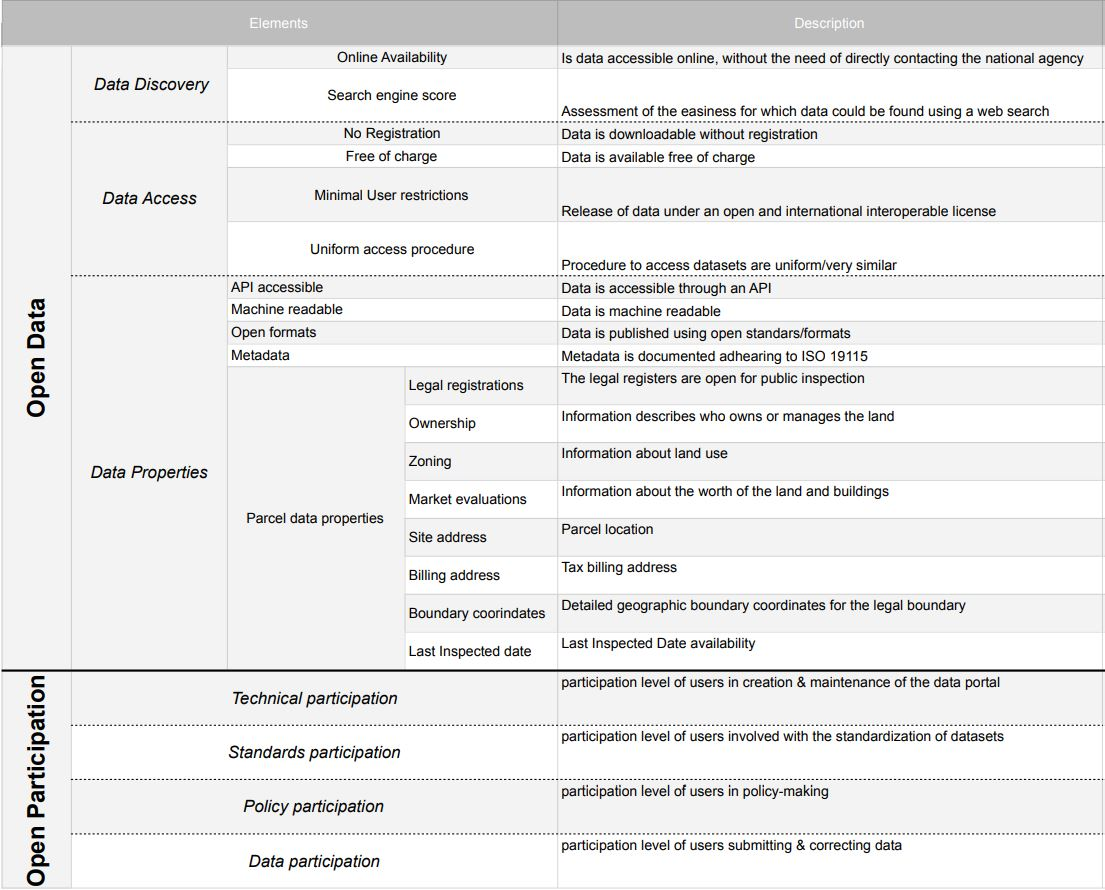
\includegraphics[width=20cm]{images/assessment_framework_description.JPG}
    \caption{The full assessment framework}
    \label{fig:assesment_result}
\end{figure}